\documentclass[a4paper,11pt]{article}
\usepackage[utf8]{inputenc}

\title{Notes}
\author{Tiarnán Curran-Feeney}
\date{June 2021}

\usepackage[ruled,vlined]{algorithm2e}
\usepackage[numbers]{natbib}
\bibliographystyle{plainnat}
\usepackage{cite}

\usepackage{amsmath}
\usepackage{amsfonts}
\usepackage{amssymb}

\usepackage{amsthm}
\usepackage{graphicx}

\usepackage{hyperref}
\usepackage{listings}
\usepackage{color}

\usepackage{tikz}
\usetikzlibrary{shapes.geometric, arrows}
\tikzstyle{Sh} = [rectangle, rounded corners, minimum width=1cm, minimum height=1cm,text centered, draw=black, fill=green!30]
\tikzstyle{Ih} = [rectangle, rounded corners, minimum width=1cm, minimum height=1cm,text centered, draw=black, fill=red!30]
\tikzstyle{Rh} = [rectangle, rounded corners, minimum width=1cm, minimum height=1cm,text centered, draw=black, fill=blue!30]
\tikzstyle{arrow} = [thick,->,>=stealth,font=\sffamily\small]

\usepackage{array} % used for many of the table properties in this document
\usepackage{multirow} % used for the multirow commands
\usepackage{tabu} % used for the \begin{tabu}... \end{tabu} commands

\theoremstyle{plain}
\newtheorem*{game1}{Game}
\newtheorem*{wrmup}{Warm-up}
\newtheorem*{note}{Note}
\newtheorem*{game2}{Variation}
\newtheorem*{example}{Example}

\theoremstyle{definition}
\newtheorem*{goal}{GOAL}

\begin{document}

\maketitle

\begin{abstract}
    DON'T GET DISTRACTED FROM THE END GOAL:
    
    Modelling the spread of a disease between countries and looking at the distribution of resources such as vaccinations when they are in limited supply/production.
\end{abstract}

\section{Reading}

\subsection{Control}

We know from \citep{AirTravel} that the successfullness of Contact Tracing reduces the more time passes from the original event. In one example for Rubella, \citep{ControlCT}, 86\% of those exposed during shared air travel were able to be contacted. In another example with measles, \citep{ControlCTMeasles}, 81\% were successfully contacted the day after the flight landed. In \citep{AirTravel}, it was mentioned that there was a case were only 30\% were successfully contacted. Time is the key factor in successful contact tracing.

\citep{ControlEntry} concluded that entry screening is unlikely to be effective due to exposure period. It should be noted that \citep{ControlEntry} is a student article. This was summarised in \citep{AirTravel} by "entry
screening might identify an estimated 9\% of SARS cases in
England, and would not significantly affect introduction." A similar study by \citep{ControlBorder} found that no infectious individual was detected upon entry scanning at airports. This was due to a small number of infected individuals in a large population.

Isolation: "However, isolation measures are less effective if
transmission can occur while an infected person is asymptomatic" - \citep{AirTravel} was referencing: \citep{ControlLF}.

"Quarantine of contacts is expensive and requires a large
amount of resources. Models suggest that for quarantine to
be most effective in controlling influenza outbreaks, all
travelers who were on the same plane as the infected
traveler would have to be quarantined" - \citep{AirTravel} and was referencing \citep{zhang2012characteristics}. In \citep{zhang2012characteristics}, we find "The strategies of BES,
quarantine of close contacts, medical follow-up of overseas travelers, and hospital investigations
were able to detect cases efficiently albeit associated with high use of resources. A further study
on cost effectiveness of these strategies is in urgent need in the future."

One study looked at the control of Covid-19 through the isolation of cases and contacts, \citep{ControlIsolation}. A self-confessed short falling of their study was that "the model placed no
constraints on the number of cases and contacts that
could be traced and isolated." They believe the upper limit on contact tracing varies depending on the country. As would be expected, their results found that the percentage of contacts that needed to be successfully traced depends on the reproduction number. Delayed onset of symptoms is also a key factor in play. When they swapped form a short delay to a long delay it was found that "the probability of achieving
control fell from 89\% to 31\%." An area that needs improvement in their model is that they "assumed
that isolation of cases and contacts is completely
effective, and that all symptomatic cases are eventually
reported."

Control - Masks: "A “panic buying” scenario, in
which maximum demand for masks is attained very early in the
epidemic, generally had a detrimental impact on the resulting
outbreak" - see \citep{ControlFMRA}.

"One of the most notable features of human social contacts is the huge variability in the number and
strength of contacts" - \citep{WarwickCT} - For contact tracing to be effective "the time from the primary case becoming infectious to the tracing of their
contacts needs to be shorter than the incubation period"

"We find that vaccines offering relatively high protection from the first dose (compared
to the efficacy derived from two doses) favour strategies that prioritise giving more people one dose
rather than a smaller number two" - \citep{WarwickVaccCount}

\subsubsection{Vaccination}

\citep{WarwickVaccStrat} talks about the optimum method to vaccinate - may be useful to see later? Only skimmed as was 20 pages long

\citep{WarwickNonPharm} nice read but not relevant for constructing model. Maybe use for comparison later in project?


\subsection{Ethics/Economy}

\subsection{Model}

A potential local model for the dynamics of covid is the deterministic model in \citep{CovidModelIndia}. In this model we have four proposed classes Susceptible (S), Asymptomatic (A), Reported Symptomatic (I), and Unreported Symptomatic (U). This is illustrated in figure \ref{fig:determ}. The rest of article \citep{CovidModelIndia} is not of any particular interest.

\begin{figure}[hbtp]
	\centering % centers the picture horizontally
	\includegraphics[width=5in]{ModelIndia.png} % optional argument could be height = , scale = etc. and can take in units mm, cm, in, pt, em, mu,...
	\caption{Deterministic Covid Model from \citep{CovidModelIndia}.}
	\label{fig:determ}  % put the label on the caption, as this is what has been numbered.
\end{figure}

\begin{figure}[hbtp]
	\centering % centers the picture horizontally
	\includegraphics[width=5in]{ModelWarwick.png} % optional argument could be height = , scale = etc. and can take in units mm, cm, in, pt, em, mu,...
	\caption{Warwick Covid Model from \citep{WarwickNonPharm}}
	\label{fig:determ2}  % put the label on the caption, as this is what has been numbered.
\end{figure}

In \citep{ControlFMRA}, we are introduced to a particularly interesting resource allocation model. Return to this at a later date.

In \citep{ModelContactTracing}, the use of a success rate p for contact tracing along with a delay in contacting potentially exposed individuals after someone becomes detected.

\subsection{Transmission}

Transmission of diseases on commercial airplanes is of particular interest to this project. In \citep{TransAirTravel}, it is stated that "The risk of disease transmission within the confined
space of the aircraft cabin is difficult to determine.
Insufficient data prohibits meta-analysis, which would
allow an idea of the probability of disease transmission." It should be noted the same article deems an aircraft no higher risk than a office building for transmission. We should also note that the same article tells us "risk of disease transmission to other
symptom-free passengers within the aircraft cabin is
associated with sitting within two rows of a contagious
passenger for a flight time of more than 8 [hours]."

If a space is properly ventilated then "one air exchange removes 63\%
of airborne organisms," as stated in \citep{TransAirTravel}. Furthermore, "Risk also reduced exponentially to
almost zero in passengers seated 15 seats from the
infectious source." See references of \citep{TransAirTravel} for more information.

\break

\section{Plan}

\subsection{Random Notes}
Model starts with a single infection in a random country. Looking at controlling pandemics so we shall presume that it is a new virus. Hence, there is no initial vaccine available.

Each country will have a certain amount of funding, vaccine producing factories and mask producing factories. These may vary between each country. 

What do we want to be able to look at?

- Compliance to social distancing measures - 

- Rate vaccine can be produced and distributed

- Change in travel when restrictions in place

\subsection{End Goal and Motivation}

\break

\subsection{Model}

\subsubsection{Dynamics within a Country}

\begin{figure}[hbtp]
        \begin{center}
			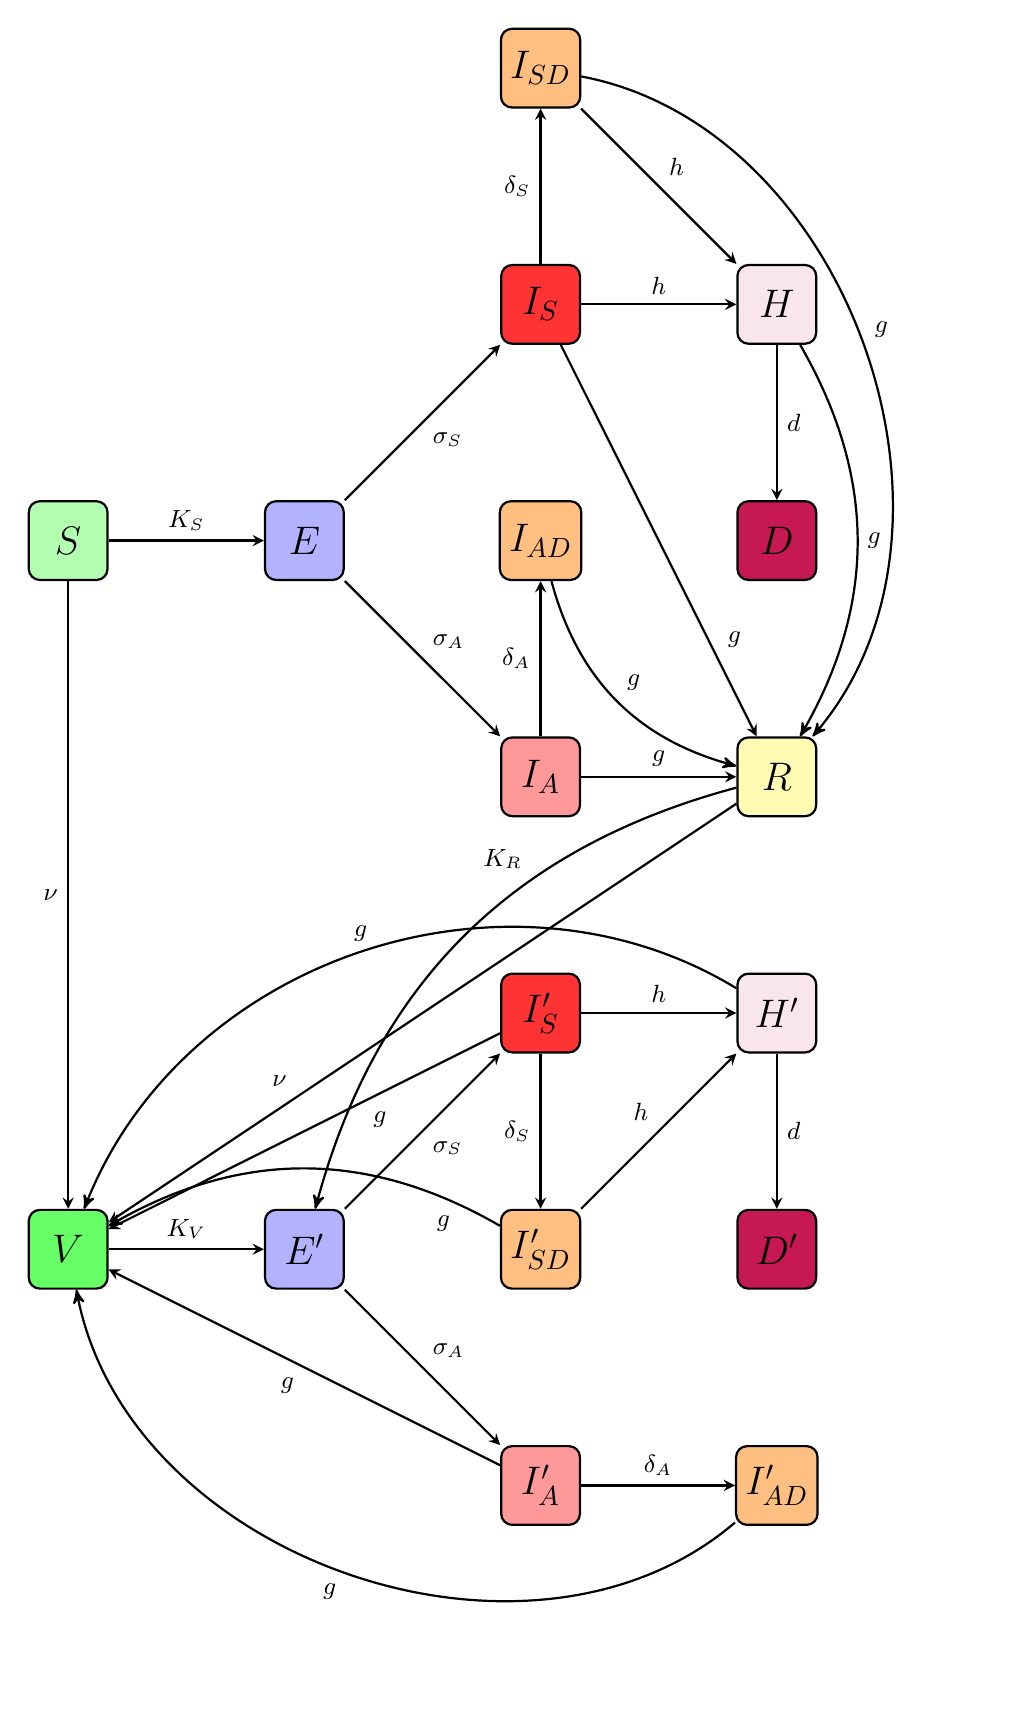
\begin{tikzpicture}[->,>=stealth',auto,node distance=3cm,
			thick,main node/.style={rectangle, rounded corners, minimum width=1cm, minimum height=1cm,text centered, draw=black,font=\sffamily\Large\bfseries},final/.style={rectangle, rounded corners, minimum width=2cm, minimum height=1cm,text centered, draw=black,font=\sffamily\Large\bfseries}]
			
			\node[main node,fill=blue!30] (4) {$E$};
			
			\node[main node,fill=green!30] (1) [left of = 4] {$S$};
			
			
			\node[main node,fill=orange!50] (5) [right of=4] {$I_{AD}$};
			
			\node[main node,fill=red!80] (6) [above of=5] {$I_S$};
			\node[main node,fill=red!40] (7) [below of= 5] {$I_A$};
			
			\node[main node,fill=orange!50] (12) [above of=6] {$I_{SD}$};
			
			
			\node[main node,fill=purple!10] (10) [right of =6] {$H$};
			
			\node[main node,fill=purple!90] (9) [below of= 10] {$D$};
			
			\node[main node,fill=yellow!30] (11) [right of= 7] {$R$};
			
			
			\node[main node,fill=purple!10] (J) [below of= 11] {$H'$};
			\node[main node,fill=purple!90] (I) [below of= J] {$D'$};
			
			\node[main node,fill=red!80] (F) [left of= J] {$I_S'$};
			\node[main node,fill=orange!50] (E) [below of=F] {$I_{SD}'$};
			\node[main node,fill=red!40] (G) [below of= E] {$I_A'$};
			
			\node[main node,fill=orange!50] (K) [right of=G] {$I_{AD}'$};
			
			\node[main node,fill=blue!30] (D) [left of=E] {$E'$};
			\node[main node,fill=green!60] (2) [left of =D] {$V$};
			
			
			\draw[arrow] (1) -- node[anchor=east] {$\nu$} (2);
			
			\draw[arrow] (1) -- node {$K_S$} (4);
			
			\draw[arrow] (4) -- node[anchor=north west] {$\sigma_S$} (6);
			\draw[arrow] (4) -- node {$\sigma_A$} (7);
			
			\draw[arrow] (6) -- node[anchor=east] {$\delta_S$} (12);
			\draw[arrow] (7) -- node {$\delta_A$} (5);
			
			%\draw[arrow] (5) -- (8);
			%\draw[arrow] (5) -- node[pos=0.6] {$d_D$} (9);
			\draw[arrow] (12) -- node {$h$} (10);
			
			\path[every node/.style={dashed,font=\sffamily\small}]
					(5) edge[bend right] node {$g$} (11)
					
					(10) edge[bend left] node {$g$} (11)
					(11) edge[bend right = 30] node[anchor=south east, pos = 0.35] {$K_R$} (D)
					(12) edge[bend left=60] node[anchor=south west] {$g$} (11);
					
		    \draw[arrow] (7) -- node {$g$} (11);
		    \draw[arrow] (6) -- node[pos=0.8] {$g$} (11);
		    
		    \draw[arrow] (6) -- node {$h$} (10);
		    %\draw[arrow] (6) -- node {$d_S$} (9);
		    %\draw[arrow] (6) -- (8);
		    
		    \draw[arrow] (10) -- node {$d$}(9);
            %\draw[arrow] (8) -- (10);
			
			
			
			\draw[arrow] (11) -- node[anchor = south east,pos=0.7] {$\nu$} (2);
			
			\draw[arrow] (2) -- node {$K_V$} (D);
			
			\draw[arrow] (D) -- node[anchor=north west] {$\sigma_S$} (F);
			\draw[arrow] (D) -- node {$\sigma_A$} (G);
			
			\draw[arrow] (F) -- node[anchor=east] {$\delta_S$} (E);
			\draw[arrow] (G) -- node {$\delta_A$} (K);
			
			\draw[arrow] (E) -- node {$h$}(J);
			
		    \draw[arrow] (F) -- node {$h$} (J);
		    %\draw[arrow] (F) -- node {$h$} (H);
		    \draw[arrow] (J) -- node {$d$} (I);

            
            \draw[arrow] (F) -- node[pos=0.35] {$g$} (2);
            \draw[arrow] (G) -- node {$g$} (2);
            
            \path[every node/.style={dashed,font=\sffamily\small}]
					(E) edge[bend right] node[pos=0.1] {$g$} (2)
					(K) edge[bend left = 60] node {$g$} (2)
					(J) edge[bend right = 50, anchor = south] node {$g$} (2);
			
			\end{tikzpicture}
		\end{center}
		\caption{Model - Detected DOESNT go to hospital as they are the detected and isolating but okay}
\end{figure}

\begin{table}[hbtp]
		\begin{center}
			\caption{Table of all transmission events.}
			\begin{tabular}{ c|c|c }
				Event & Rate & Changes \\ 
	        	\hline
		        \hline
		        Infection of Susceptible & $K_SS$ & $S \mapsto S - 1$ \\
		        &  &  $E \mapsto E + 1$\\
		        \hline
		        Infection of Vaccinated & $K_VV$ & $V \mapsto V - 1$ \\
		        &  & $E' \mapsto E' + 1$ \\
	        	\hline
	        	Infection of Recovered & $K_RR$ & $R \mapsto R - 1$ \\
	        	&  & $E' \mapsto E' + 1$ \\
			\end{tabular}
			\label{tab:E}
		\end{center}
\end{table}

$K_J = \beta_J (\alpha_E E + \alpha_D I_D + \alpha_A I_A + \alpha_S I_S + \kappa_E E' + \kappa_D I_D' + \kappa_A I_A' + \kappa_S I_S')$
	
\begin{table}[hbtp]
		\begin{center}
		    \caption{Table of all transition events for Non-Vaccinated Individuals.}
			\begin{tabular}{ c|c|c }
				Event & Rate & Changes \\ 
	        	\hline
		        \hline
	            Exposed Becomes Asymptomatic & $\sigma_AE$ & $E \mapsto E - 1$  \\
	            & & $I_A \mapsto I_A + 1$\\
	            \hline
	            Exposed Becomes Symptomatic & $\sigma_SE$ &  $E \mapsto E - 1$ \\
	            &  & $I_A \mapsto I_S + 1$\\
	            \hline
	            Symptomatic Becomes Detected & $\delta_SI_S$ & $I_S \mapsto I_S - 1$  \\
	            & & $I_{SD} \mapsto I_{SD} + 1$\\
	            \hline
	            Asymptomatic Becomes Detected & $\delta_A I_A$ & $I_A \mapsto I_A - 1$  \\
	            &  & $I_{AD} \mapsto I_{AD} + 1$\\
	            \hline
		        Asymptomatic Recovers & $g I_A$ & $I_A \mapsto I_A - 1$  \\
	            &  & $R \mapsto R + 1$\\
	            \hline
	            Detected Recovers & $g I_{SD}$ & $I_{SD} \mapsto I_{SD} - 1$ \\
	             &  & $R \mapsto R + 1$\\
	            \hline
	            Detected Recovers & $g I_{AD}$ & $I_{AD} \mapsto I_{AD} - 1$ \\
	             &  & $R \mapsto R + 1$\\
	            \hline
	            Detected Hospitalised & $h I_{SD}$ & $I_{SD} \mapsto I_{SD} - 1$ \\
	             &  & $H \mapsto H + 1$\\
	            \hline
	            Symptomatic Recovers & $g I_S$ & $I_S \mapsto I_S - 1$ \\
	            &  & $R \mapsto R + 1$\\
	            \hline
	            Symptomatic Hospitalised & $h I_S$ &  $I_S \mapsto I_S - 1$\\
	            &  & $H \mapsto H + 1$\\
	            \hline
	            Hospitalised Recovers & $g H$ & $H \mapsto H - 1$\\
	             &  & $R \mapsto R + 1$\\
	            \hline
	            Hospitalised Dies & $d H$ & $H \mapsto H - 1$\\
	            &  & $D \mapsto D + 1$\\
	            \hline
	            Susceptible Vaccinated & $\nu$ &  $S \mapsto S - 1$\\
	            &  & $V \mapsto V + 1$\\
	            \hline
	            Recovered Vaccinated & $\nu$ &  $R \mapsto R - 1$\\
	            &  & $V \mapsto V + 1$\\
			\end{tabular}
			\label{tab:A}
		\end{center}
	\end{table}
	
\begin{table}[hbtp]
		\begin{center}
		    \caption{Table of all transition events for Vaccinated Individuals.}
			\begin{tabular}{ c|c|c }
				Event & Rate & Changes \\ 
	        	\hline
		        \hline
	            Exposed Becomes Asymptomatic & $\sigma_A E'$ & $E' \mapsto E' - 1$  \\
	            & & $I_A' \mapsto I_A' + 1$\\
	            \hline
	            Exposed Becomes Symptomatic & $\sigma_SE'$ &  $E' \mapsto E' - 1$ \\
	            &  & $I_S' \mapsto I_S' + 1$\\
	            \hline
	            Symptomatic Becomes Detected & $\delta_SI_S'$ & $I_S' \mapsto I_S' - 1$  \\
	            & & $I_{SD}' \mapsto I_{SD}' + 1$\\
	            \hline
	            Asymptomatic Becomes Detected & $\delta_A I_A'$ & $I_A' \mapsto I_A' - 1$  \\
	            &  & $I_{AD}' \mapsto I_{AD}' + 1$\\
	            \hline
		        Asymptomatic Recovers & $g I_A'$ & $I_A' \mapsto I_A' - 1$  \\
	            &  & $V \mapsto V + 1$\\
	            \hline
	            Detected Recovers & $g I_{SD}'$ & $I_{SD}' \mapsto I_{SD}' - 1$ \\
	             &  & $V \mapsto V + 1$\\
	            \hline
	            Detected Recovers & $g I_{AD}'$ & $I_{AD}' \mapsto I_{AD}' - 1$ \\
	             &  & $V \mapsto V + 1$\\
	            \hline
	            Detected Hospitalised & $h I_{SD}'$ & $I_{SD}' \mapsto I_{SD}' - 1$ \\
	             &  & $H' \mapsto H' + 1$\\
	            \hline
	            Symptomatic Recovers & $g I_S'$ & $I_S' \mapsto I_S' - 1$ \\
	            &  & $V \mapsto V + 1$\\
	            \hline
	            Symptomatic Hospitalised & $h I_S'$ &  $I_S' \mapsto I_S' - 1$\\
	            &  & $H' \mapsto H' + 1$\\
	            \hline
	            Hospitalised Recovers & $g H'$ & $H' \mapsto H' - 1$\\
	             &  & $V \mapsto V + 1$\\
	            \hline
	            Hospitalised Dies & $d H'$ & $H' \mapsto H' - 1$\\
	            &  & $D' \mapsto D' + 1$\\
	            \hline
			\end{tabular}
			\label{tab:B}
		\end{center}
	\end{table}

\begin{table}[hbtp]
		\begin{center}
			\caption{Table of all Travel events.}
			\begin{tabular}{ c|c|c }
				Event & Rate & Changes \\ 
	        	\hline
		        \hline
		        Susceptible from country j travels to country i & $\epsilon_{ij} S_{jj}$ & $S_{jj} \mapsto S_{jj} - 1$ \\
		        &  &  $S_{ij} \mapsto S_{ij} + 1$\\
		        \hline
		        Exposed from country j travels to country i & $\epsilon_{ij} E_{jj}$ & $E_{jj} \mapsto E_{jj} - 1$ \\
		         &  &  $E_{ij} \mapsto E_{ij} + 1$\\
		        \hline
		        Asymptomatic from country j travels to country i & $\epsilon_{ij} I_{Ajj}$ & $I_{Ajj} \mapsto I_{Ajj} - 1$ \\
		        &  &  $I_{Aij} \mapsto I_{Aij} + 1$\\
	        	\hline
	        	Symptomatic from country j travels to country i & $\epsilon_{ij} I_{Sjj}$ & $I_{Sjj} \mapsto I_{Sjj} - 1$ \\
		        &  &  $I_{Sij} \mapsto I_{Sij} + 1$\\
	        	\hline
	        	Recovered from country j travels to country i & $\epsilon_{ij} R_{jj}$ & $R_{jj} \mapsto R_{jj} - 1$ \\
		        &  &  $R_{ij} \mapsto R_{ij} + 1$\\
	        	\hline
	        	Vaccinated from country j travels to country i & $\epsilon_{ij} V_{jj}$ & $V_{jj} \mapsto V_{jj} - 1$ \\
		        &  &  $V_{ij} \mapsto V_{ij} + 1$\\
	        	\hline
	        	Exposed from country j travels to country i & $\epsilon_{ij} E'_{jj}$ & $E'_{jj} \mapsto E'_{jj} - 1$ \\
		        &  &  $E'_{ij} \mapsto E'_{ij} + 1$\\
	        	\hline
	        	Asymptomatic from country j travels to country i & $\epsilon_{ij} I'_{Ajj}$ & $I'_{Ajj} \mapsto I'_{Ajj} - 1$ \\
		        &  &  $I'_{Aij} \mapsto I'_{Aij} + 1$\\
	        	\hline
	        	Symptomatic from country j travels to country i & $\epsilon_{ij} I'_{Sjj}$ & $I'_{Sjj} \mapsto I'_{Sjj} - 1$ \\
		        &  &  $I'_{Sij} \mapsto I'_{Sij} + 1$\\
                \hline
		        Susceptible from country j in country i returns home & $\epsilon_{ji} S_{ij}$ & $S_{ij} \mapsto S_{ij} - 1$ \\
		        &  &  $S_{jj} \mapsto S_{jj} + 1$\\
		        \hline
		        Exposed from country j in country i returns home & $\epsilon_{ji} E_{ij}$ & $E_{ij} \mapsto E_{ij} - 1$ \\
		        &  &  $E_{jj} \mapsto E_{jj} + 1$\\
		        \hline
		        Asymptomatic from country j in country i returns home & $\epsilon_{ji} I_{Aij}$ & $I_{Aij} \mapsto I_{Aij} - 1$ \\
		        &  &  $I_{Ajj} \mapsto I_{Ajj} + 1$\\
		        \hline
		        Symptomatic from country j in country i returns home & $\epsilon_{ji} I_{Sij}$ & $I_{Sij} \mapsto I_{Sij} - 1$ \\
		        &  &  $I_{Sjj} \mapsto I_{Sjj} + 1$\\
		        \hline
		        Recovered from country j in country i returns home & $\epsilon_{ji} R_{ij}$ & $R_{ij} \mapsto R_{ij} - 1$ \\
		        &  &  $R_{jj} \mapsto R_{jj} + 1$\\
		        \hline
		        Vaccinated from country j in country i returns home & $\epsilon_{ji} V_{ij}$ & $V_{ij} \mapsto V_{ij} - 1$ \\
		        &  &  $V_{jj} \mapsto V_{jj} + 1$\\
		        \hline
		        Exposed from country j in country i returns home & $\epsilon_{ji} E'_{ij}$ & $E'_{ij} \mapsto E'_{ij} - 1$ \\
		        &  &  $E'_{jj} \mapsto E'_{jj} + 1$\\
		        \hline
		        Asymptomatic from country j in country i returns home & $\epsilon_{ji} I'_{Aij}$ & $I'_{Aij} \mapsto I'_{Aij} - 1$ \\
		        &  &  $I'_{Ajj} \mapsto I'_{Ajj} + 1$\\
		        \hline
		        Symptomatic from country j in country i returns home & $\epsilon_{ji} I'_{Sij}$ & $I'_{Sij} \mapsto I'_{Sij} - 1$ \\
		        &  &  $I'_{Sjj} \mapsto I'_{Sjj} + 1$\\
			\end{tabular}
			\label{tab:C}
		\end{center}
\end{table}

\break

\section{Progress}

\subsection{Week 1}

Focus:

SIR type metapop model - Groups travelling

Find out percentage of people who travel a lot

Don't add things in without knowledge on it

Don't tie too hard to covid

testing prior to travel

SIR type model - or SIAR model?

Vaccination class how? Vaguely model based on how it currently is?

Movement between countries can be found out

Wealth of country, do they produce vaccines etc...

Partial immunity not full immunity from vaccine? ~ perhaps works?

health benefits, deaths, metric for how good or bad

DALYS how, deaths how, 

Do people permanantly move or do they commute back and forth? - Movement Matrix

THIS WEEK'S PLAN:
type up model plan and code it up ~ quality


\subsubsection{Monday}

Read a few articles and thought more about the end goal of the project. Progress today was slower than expected. In regards coding the model, I decided the best decision would be a Tauleap algorithm as would work best in terms of encorporating scheduled flights into the model.

Goal for tomorrow: Modify Tauleap model code from MA4M1 to suit this project.

\subsubsection{Tuesday}

Started constructing a model. Since this is for a general future outbreak we want a model capable of adapting to the given disease. Hence in each region we will have multiple classes and a transition matrix that can be modified to indicate the rate of transition between each class and include (or exclude) an asymptomatic infectious period before symptoms onset etc...

PROPOSAL: We have certain number of planes flying out of a country on a given day. Each plane has a maximum capacity, C. The number of people on each plane will be between 0 and C. The people will be randomly selected from the population. At the start of the day (ie before transmissions are updated) individuals on the plane are moved to a new set of classes to represent their flight. At the end of the day, after transmissions have been updated, the individuals will be moved to the classes of the new country they travelled to. This will allow us to attempt to consider transmission aboard the plane as well.

Need to get a reliable source on transmission on long flights. We will assume that people only travel via air between countries for now. This is an inaccurate assumption but can be corrected at a later date.

Progress (time 11:22): Made minor changes to Tau Leap code. Still needs to be finished.

Progress (time 15:55): Finished editing code to run N separate outbreaks independently. Need to add in travel between countries to finish it off.

Goal for Tomorrow: Do more reading, select a specific model for the project, code air travel between countries [Maybe too many tasks but choose from this list for tomorrow!]

\subsubsection{Wednesday}

Progress (time 9:36): Tested code from yesterday. Appears to be working for one country. Will try with 3 countries. Still need to add travel between countries. - Code is slow due to looping when Tau Leap fails but this can be sorted later

Progress (time 11:10): Attempted to implement some sort of code that could eventually be used for travel between countries. Progress is a little slow. Contemplating trying a different method for travel.

Progress (time 13:34): took a cheekily long lunch break and started back at the coding

End of day: Slow progress - getting my head around the code slowed me down

Goal for tomorrow: put together diagrams and have work ready to present for meeting at 2

\begin{figure}
    \begin{center}
	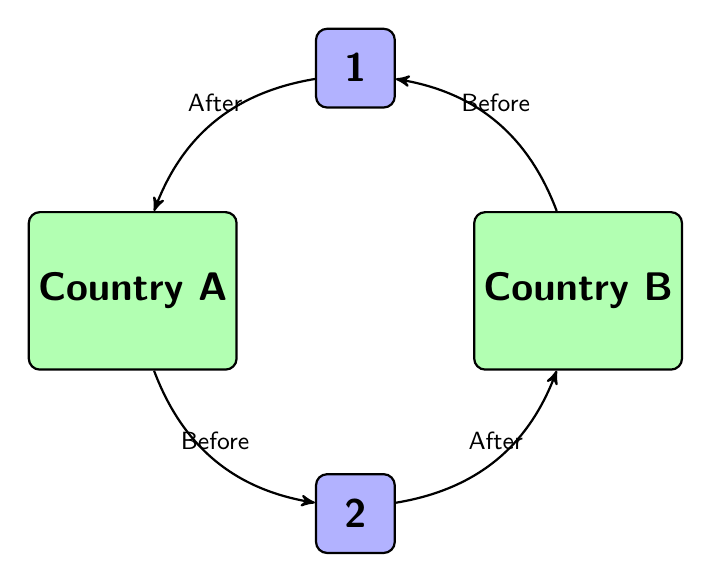
\begin{tikzpicture}[->,>=stealth',auto,node distance=4cm,
	thick,main node/.style={rectangle, rounded corners, minimum width=1cm, minimum height=2cm,text centered, draw=black,font=\sffamily\Large\bfseries}, plane/.style={rectangle, rounded corners, minimum width=1cm, minimum height=1cm,text centered, draw=black,font=\sffamily\Large\bfseries}]
	
	\node[main node,fill=green!30] (1) {Country A};
	
	\node[plane,fill=blue!30] (3) [above right of=1] {1};
	\node[plane,fill=blue!30] (4) [below right of=1] {2};
	
	\node[main node,fill=green!30] (2) [below right of=3] {Country B};
	
	\path[every node/.style={dashed,font=\sffamily\small}]
	(1) edge[bend right] node [right,anchor=south] {Before} (4)
	(2) edge[bend right] node [right,anchor=south] {Before} (3)
	(3) edge[bend right] node [left,anchor=south] {After} (1)
	(4) edge[bend right] node [left,anchor=south] {After} (2);
	\end{tikzpicture}
	\end{center}
	\caption{Travel of individuals between countries. "Before" indicates that the movement of people from the country onto the plane occurs before the tau leap step. "After" indicates that the movement of people from the plane to the country occurs after the tau leap step.}
	\label{test}
\end{figure}

\subsubsection{Thursday}

Progress (time 12:11): Started working on the project late today. Put together a Tikz diagram of a modified version of the Warwick model from \citep{WarwickNonPharm} to potentially use for the project.

Progress (time 13:49): Fixed bug with code for transition matrix

Notes:
- Do we want people to become part of population when they travel? Depends on the type of disease whether we care or not. Consider having people separate from population? Explain how movement works.

- Write up events table. 

- Consider not worrying about plane travel! Keeping it simpler for now

- How do countries want to deal with fair resource sharing when people coming in are dangerous to them?

\subsubsection{Friday}

Read notes on commuter model - plan today is to modify code to work for commuter rather than permanent movement

Infection events updated (but untested) need to sort transition events.

Transition Events now updated. Code still needs to be rigorously tested but appears to work (ie runs without spitting errors at me).

After slightly more testing appears to work well. Couple issues found and fixed. So we now have populations in each country divided into groups depending on their home country. Travelling between countries is not yet set up.

\subsubsection{Sunday}

Plan is to finish base code in time for Monday. Need to implement movement between countries. A little tricky to do however *hopefully* it is now set up. I just need to swap the matrices around until it performs the correct multiplication. Got confused around order of matrices - taking a break.

\subsection{Week 2}

Monday-Saturday were taken off while away in London.

\subsubsection{Sunday}

Movement code tested in full and is working!

Questions for Monday:
- Should a person from country i residing in country j travel to country k at the rate individuals in country i travel to k or the rate individuals from country j travel to country k ~ go from A to B to A

- Assumptions about travel regarding who can move?

- 4th year project

- Restriction levels - normal, semi, full

- Imposter Syndrome

- Look at small problem E.G: UK + ROI + Outside world

\subsection{Week 3}

\subsubsection{Monday}

Meeting to discuss progress. Fixed up diagram.

Notes from meeting:

Commuter model - travel from A to B to A to C not A to B to C

Separate rates into transmission, transition, and travel

Split up and elaborate on events table

Detected go to hospital, die etc...

vaccine is lifelong

Do inf return to sus? ~ Recovery go to vaccinated class

UK, Ireland, 



TO DO:
Find number of vaccines given daily per country

Graphical representation - graphs and maybe space/map representations ~ Maybe download shape file to colour in maps (do this later)




%Stochastic Processes, Approximations and Randomised Algorithms

%PhDs apply early ie October/November

%Cancer Research UK? Public Health England? Consider grad programmes

%NO PANIC BUT ALSO PANIC

%R Project matters - Epi Modelling

\subsubsection{Tuesday}

Added in rates to tables. Still need to do Travel Events. Started fixing code for travel so that someone from country i in country j can only move back to i. This has potentially been fixed!

Vaccines implemented with a max number allowed to be given per day - Only given to those who live in the country.

\subsubsection{Wednesday}

Created variety of different basic display for results - shows change through time for each country.

\subsubsection{Friday}

Finished up event tables

Changed code to allow for different transmission rates in different countries

Plan for rest of day is to find info on daily vaccination rate uk/Ireland and general travel rate between them

Vaccine Roll Out started in ROI 29th December 2020 - By 22nd July 5,437,340 vaccines administered (205 days) -- ie 26,524 on average a day

Vaccine Roll Out started in Britain on 8th December - By 22nd July 81,023,676 vaccines administered (225 days) -- ie 360,105 on average a day

Vaccine Roll Out started in NI on 8th December - By 22nd July 2,195,815 vaccines administered (225 days) -- ie 9,759 on average a day

Wales first dose 2,285,118
Scotland 3,992,327
NI 1,192,181
England 39,007,219

SECOND DOSE
Wales 1,959,641
Scotland 3,044,803
NI 1,003,634
England 30,754,568

WALES TOTAL: 4,244,759
SCOTLAND TOTAL: 7,037,130
ENGLAND TOTAL: 69,761,787

BRITAIN TOTAL: 81,023,676

\subsubsection{Saturday}

Implemented model into code - factored in daily vaccination rate etc...

\subsection{Week 4}

\subsubsection{Monday}

Notes from session:

Llambda

Add two detected classes - :)
Change gamma to something else 

Get rid of U to simplify things (add dH)

sigmaS + sigmaA add to rate leaving E
could write as sigma*pS and sigma(1-pS)

higher asymptomatic among vaccinated/recovered - R goes to E' maybe?

different sigma and h for V class - try trial data? Astrazeneka/Physier

Find how does vaccination change hospitalised/death prob compared to unvaccinated

keep D, D' separate

listing what the parameter is in the model find data for the parameters reference sources

Put vaccine country info into table format - max possible per day etc...

rapidly adapt and deploy - short delay on vaccination roll out

\begin{table}[hbtp]
		\begin{center}
			\caption{Table Showing Country Vaccination Information as of 22nd July.}
			\begin{tabular}{ c|c|c|c }
				Country & First Doses & Second Doses & Total Doses \\ 
	        	\hline
		        \hline
		        ROI & First Doses & Second Doses & 5,437,340 \\ 
		        \hline
		        England & 39,007,219 & 30,754,568 & 69,761,787\\ 
		        \hline
		        Scotland & 3,992,327 & 3,044,803 & 7,037,130 \\ 
		        \hline
		        Wales & 2,285,118 & 1,959,641 & 4,244,759 \\ 
		        \hline
		        NI & 1,192,181 & 1,003,634 & 2,195,815 \\ 
		        \hline
		        Britain & 45,284,664 & 35,759,012 & 81,043,676 \\ 
			\end{tabular}
			
			\begin{tabular}{ c|c|c|c }
				Country & First Vaccination Day & Average Doses/Day & Most Doses Given in a Day \\ 
	        	\hline
		        \hline
		        ROI & 29/12/20 & 26,524 & unknown\\ 
		        \hline
		        England & 08/12/20 &  308,680 & 756,873\\ 
		        \hline
		        Scotland & 08/12/20 &  31,138 & 65,249\\ 
		        \hline
		        Wales & 08/12/20 &  18,782 & 40,211\\ 
		        \hline
		        NI & 08/12/20 & 9,716 & 31,972 \\ 
		        \hline
		        Britain & 08/12/20 & 358,600 & 844,285 \\ 
			\end{tabular}
			\label{tab:L}
		\end{center}
\end{table}

\subsubsection{Tuesday}

Finished Table \ref{tab:L}.

\bibliography{Biblio}

\end{document}
